\section{Event selection}
\label{sec:dihiggs_selection}
%-------------------------------------------------------------------------------

The final state of interest consists of one charged lepton, one neutrino, 
and four quarks, two of which are b-quarks. Hence the detector signature
consists of one  charged lepton ($e$/$\mu$), large $\met$, and four or more
anti-$k_t$ jets of which two are $b$ jets from the $h$ decay while the other
two are light jets from the hadronic decay of the $W$ boson. One challenge
in the event reconstruction is to correctly identify the pair of light jets
from the $W$ boson decay. This information is also used to solve for the $z$
component of the neutrino momentum. For the $hh$ signal there is additional
complication due to the fact that one of the 
$W$ bosons is off-shell, and thus for this $W$ there is no $W$ mass constraint. 
This section details the stages of the event reconstruction and the
progression towards the final selection which defines the signal
region.  In addition, signal depleted control regions are defined in the
next section which are used to check the consistency of the SM background
predictions with the data in the control regions. The search
has been kept ``blinded'' until the comparison between data and
simulation of backgrounds are well understood in the signal depleted
control regions.

\subsection{Trigger requirement}

For data collected in 2015 and 2016, the trigger requires the presence of at least one lepton. 
%The muon trigger requires a $p_T > 20$ GeV
%muon and it is  seeded by a $p_T > 15$ GeV Level-1 trigger while
%the electron trigger requires a $p_T > 24$ GeV electron  and is seeded by a $p_T >
%20$ GeV trigger at Level-1. Loose isolation is required at trigger
%level.  
The specific triggers are a logical OR of HLT\_e24\_lhmedium\_iloose\_L1EM18VH, HLT\_mu20\_iloose\_L1MU15 in data collected in 2015, and for data collected in 2016 it is the logical OR of HLT\_e24\_lhtight\_nod0\_ivarloose, HLT\_E60\_lhmedium\_nod0, HLT\_mu24\_iloose(data), or HLT\_mu24\_L1Mu15 (MC).


\subsection{Event pre-selection}

The following selection cuts are applied at the pre-selection level to the recorded events:
\begin{itemize}
\item In order to assure good data quality, events with bad detector
  conditions, namely where large part of the detectors were missing
  from data acquisition due to problems during a run, or when the
  performance of the detectors were affected by large noise, have been
  rejected from the data analysis. A GRL selection taken from
       data15\_13TeV.periodAllYear\_DetStatus-v73-pro19-08\_DQDefects-00-01-02\_PHYS\_StandardGRL\_All\_Good\_25ns.xml
       or data16\_13TeV.periodAllYear\_DetStatus-v81-pro20-10\_DQDefects-00-02-02\_PHYS\_StandardGRL\_All\_Good\_25ns.xml
   ~\cite{GRL}       is applied, moreover events are rejected if:
       eventInfo->errorState(xAOD::EventInfo::EventFlagSubDet::Tile)==
       xAOD::EventInfo::Error,
       eventInfo->errorState(xAOD::EventInfo::EventFlagSubDet::LAr)== 
xAOD::EventInfo::Error,
eventInfo->errorState(xAOD::EventInfo::EventFlagSubDet::SCT)== 
xAOD::EventInfo::Error, (eventInfo->eventFlags(EventInfo::Core) \& 0x40000) is true to
	avoid incomplete events.
 
\item the presence of a  primary vertex with at least two
  tracks. Among all primary vertices, that with the highest
	 $\sum p_{{\rm T,trk}}^{2}$, where
	$p_{{\rm T,trk}}$ is the transverse momentum of tracks
	associated with the vertex, is retained as the primary
        interaction vertex.
\item at least one $e$ or $\mu$.
\item at least 4 jets, of which  2 and only 2 are $b$-tagged.
\end{itemize}


\subsection{Event Reconstruction}
%%The final state of our signal consists of one charged lepton, one neutrino, and four quarks, 
%%two being $b$-quraks. Hence the detector signature consists of one charged lepton, missing 
%%transverse momentum, and four or more jets of which two are $b$ jets from the $h$ decay while 
%%the other two are light jets from the hadronic decay of the $W$ boson. 
Events are reconstructed by first requiring two 2 $b$-tag jets and at least two light
jets and at most 3 light jets. In events with 3 light jets, the pair with the 
lowest $\Delta R$ between them are selected as $W$ jet candidates. This
procedure yields the correct jet assignment in 70 \% of the cases where the
hadronic daughters of the $W$ boson can be correctly matched to reconstructed
jets as described in Appendix~\ref{app:jetTruthStudies}.
%After preselection both light jets from $W$ bosons can be correctly matched in  20 \% of events.(see Appendix \ref{sec:BenStudy}).  

The event kinematics of the $h \to WW^* \to l \nu qq$ topology can be fully
reconstructed. In fact, among all four-momenta of the final state particle,
only the component of the neutrino momentum along the beam axis, the neutrino
longitudinal momentum in the following, is unknown while its transverse
momentum is the measured $\met$. Imposing the relation:
\begin{equation}
\label{eq:mh}
m_h^2 = (p^l + p^{\nu} + p^{j1} + p^{j2})^2
\end{equation}
where $p^i$ is the four-momenta of particle $i$ the neutrino $p_z$ can be
reconstructed by the relations:
\[
p_E^{\nu} = E^{\nu} = \sqrt{P_T^2 + p_z^2} \quad p_x^{\nu} = P_Tcos(\phi) \quad p_y^{\nu} = P_T sin(\phi)
\]
where $\phi$ is the azimuthal angle of the $\met$, $E^{\nu}$ the neutrino
energy and $p_x$ and $p_y$ the two spatial components of the neutrino momentum.
Eq. \ref{eq:mh} is a quadratic expression in $p_z$. It can have two real,
one real  or two complex solutions. In the last case only the real part of the
complex solution is taken into account, therefore a single value of $p_z$ is
obtained. In the first case the solution with the neutrino direction closest
to the charged lepton is retained. It has been shown that this algorithm
selects the correct solution in approximately 60\% of the cases
(see Appendix \ref{app:nupz_studies}).


\subsection{Kinematic selection}
\label{subsec:kincuts}


Kinematic selection is used to suppress mainly $t\bar{t}$ background with
respect to the signal.  A schematic of the $hh \to WWbb$ and the
$t \bar{t} \to WWbb$ event topology is shown in Figure \ref{fig:cartoon}.
\begin{figure}
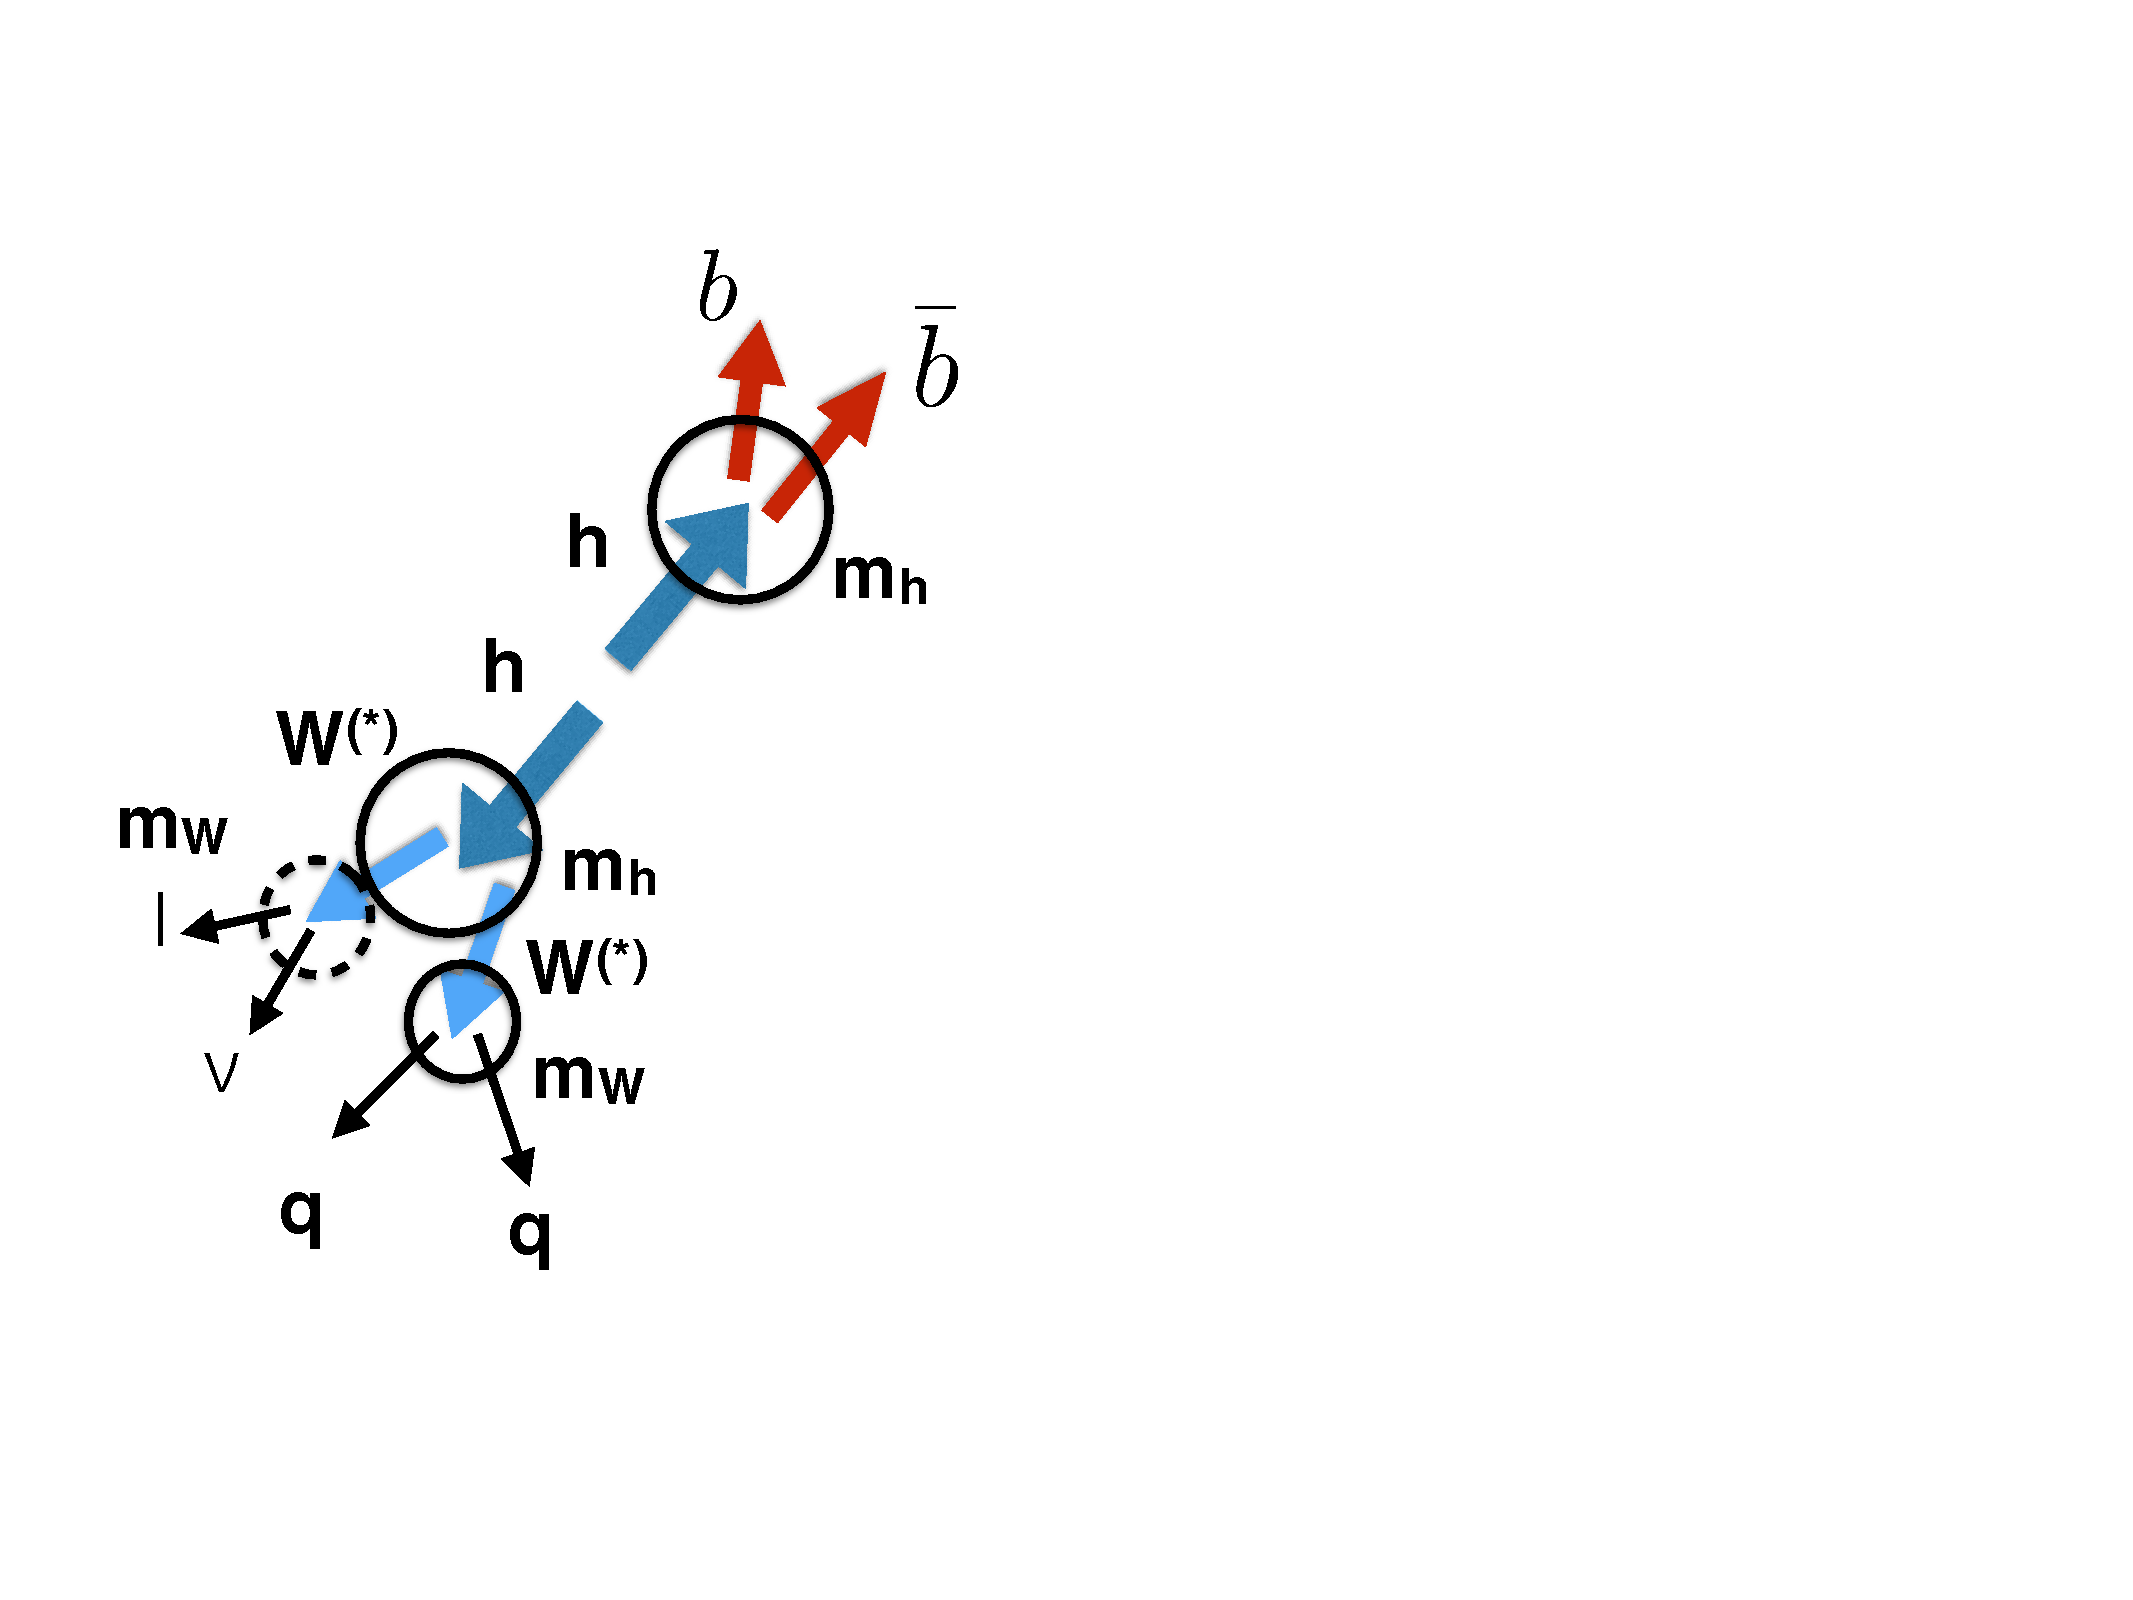
\includegraphics[width=0.5\textwidth]{chapters/dihiggs/figures/cartoon_hh.pdf}
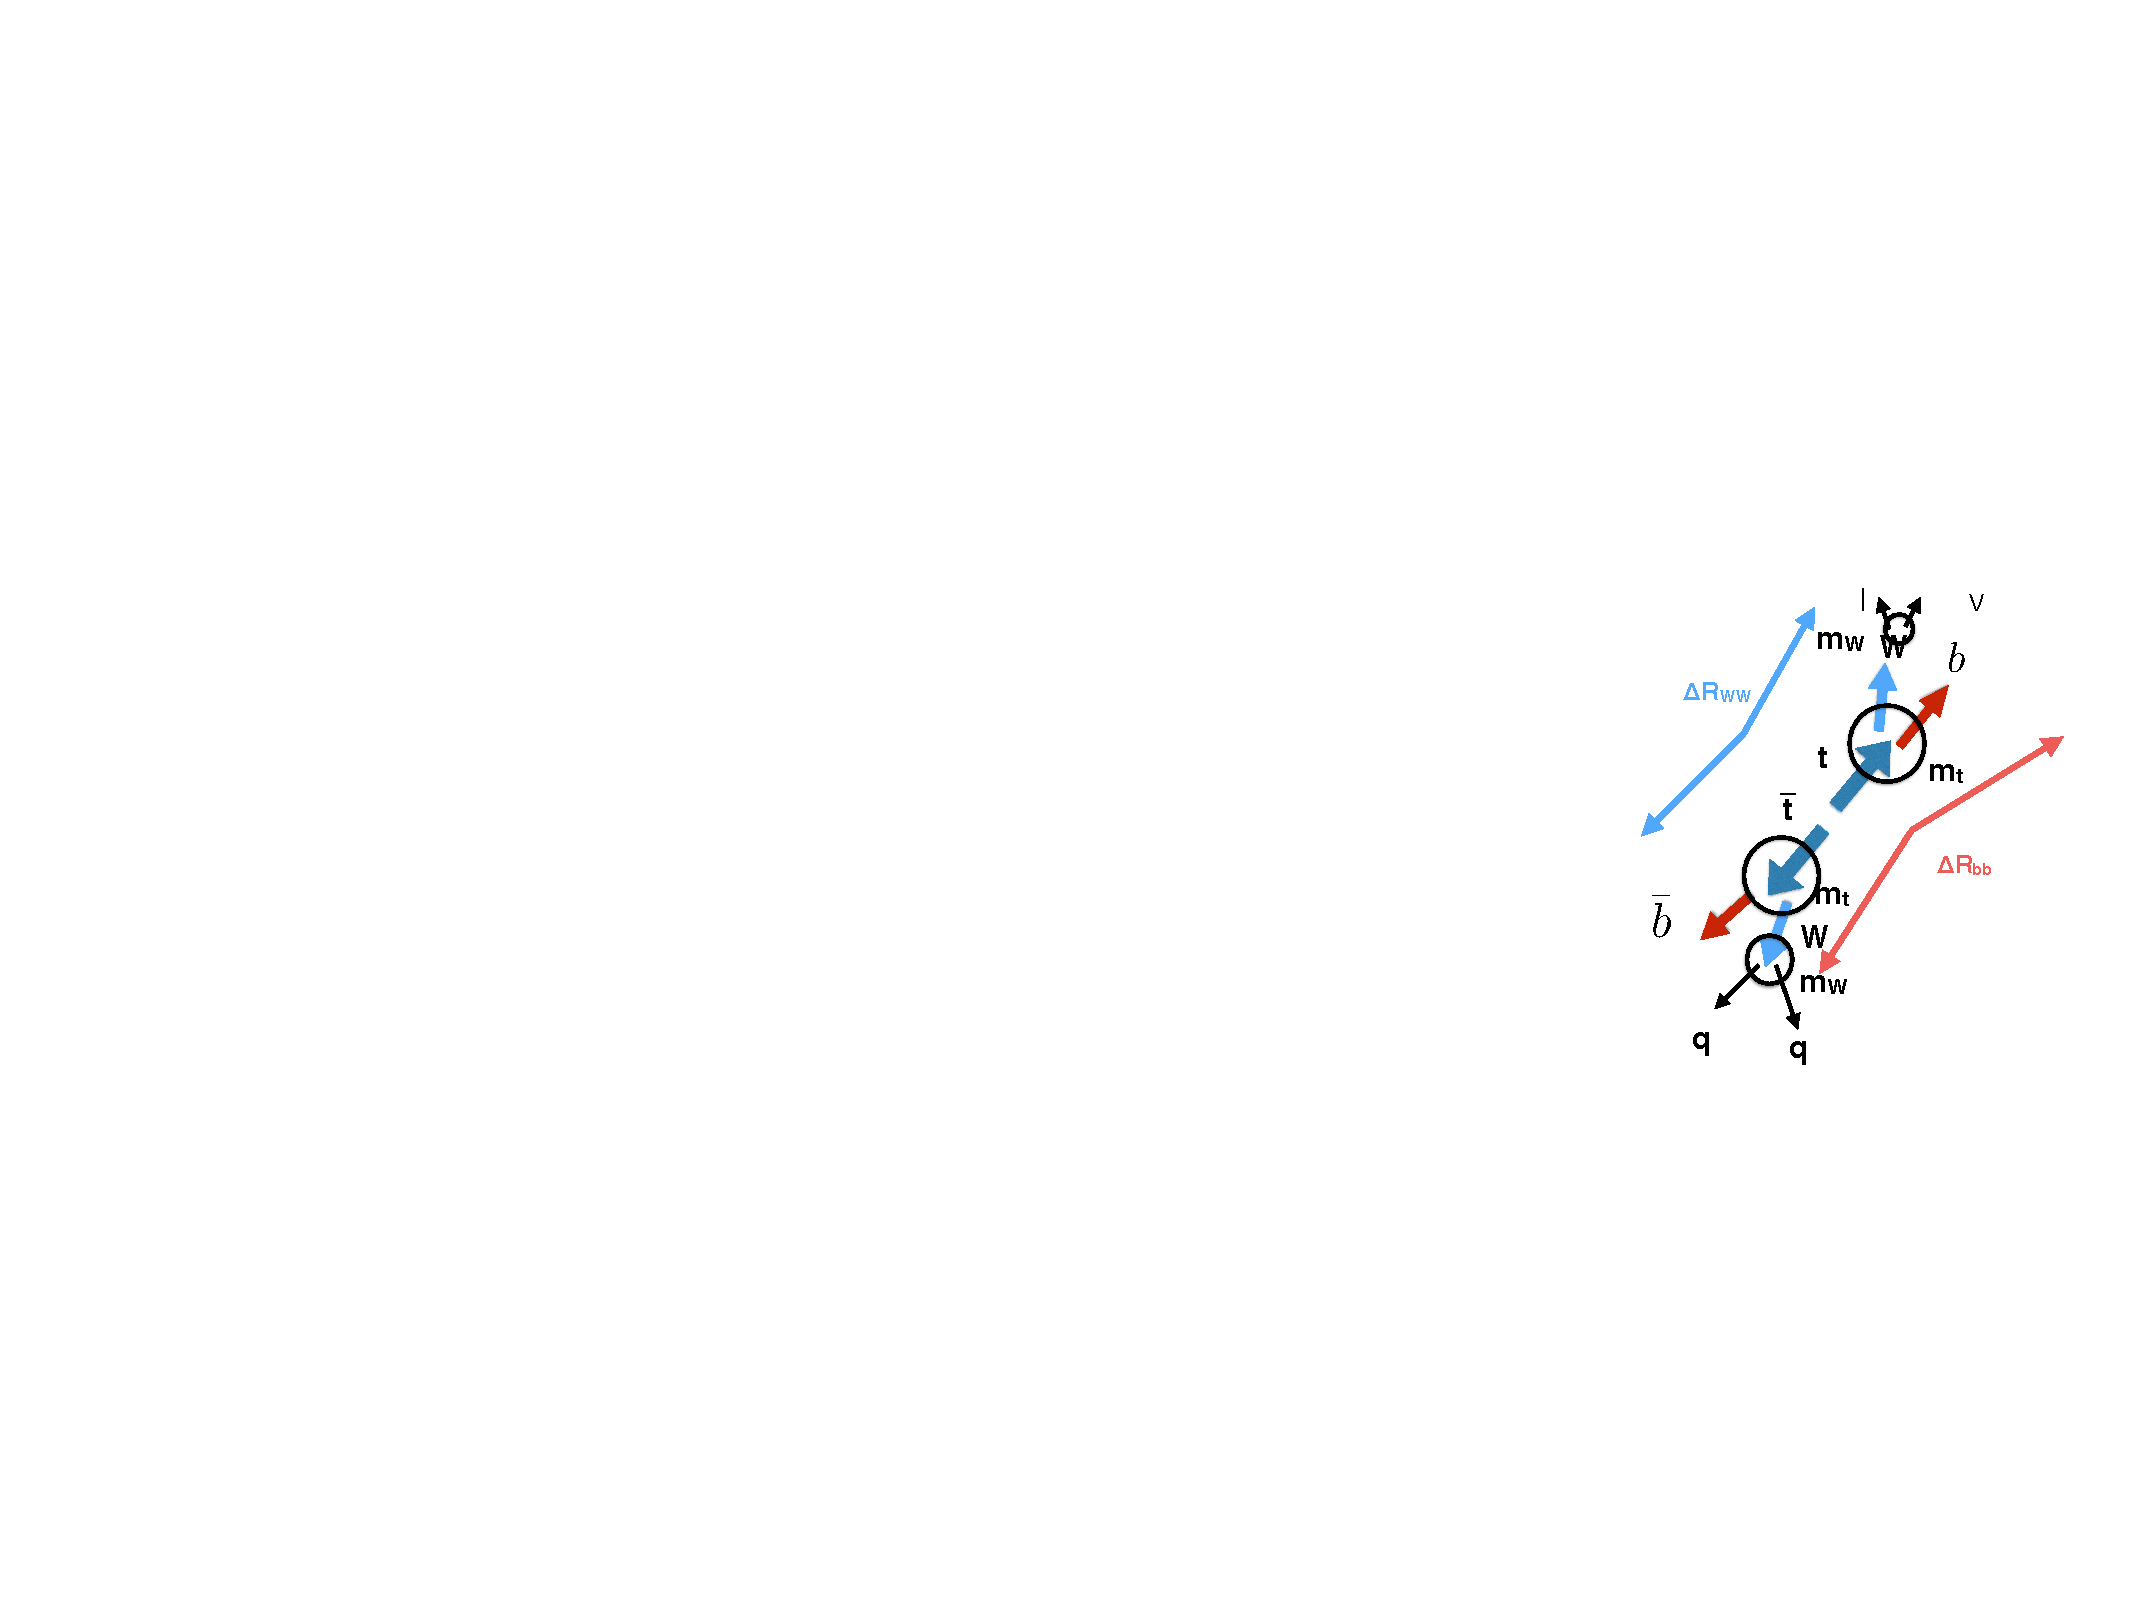
\includegraphics[width=0.5\textwidth]{chapters/dihiggs/figures/cartoon_tt.pdf}
\caption{Schematic view of a $hh \to WWbb$ event compared to a $t\bar{t} \to WWbb$ event.} 
\label{fig:cartoon}
\end{figure}

The $t \bar{t}$ events are typically characterised by two $b$-jets and
two $W$ bosons such that the $\Delta R$ separation between the $b$-jets
with each other is large, and similarly the $\Delta R$ separation between
the $W$ bosons with each other is also large. On the contrary, in particular
when the invariant mass of the $m_{hh}$ is high, the signal is characterised
by two $b$-jets which are close together in $\Delta R$ and by two $W$ bosons
which are also relatively closer. Moreover, while in the signal 
case the two $b$-jets have an invariant mass equal to $m_h$, this is not
the case for the $t \bar{t}$ background, where an almost continuous
distribution is expected.  Following these, the typical separation variables are: 
\begin{itemize}
\item the $p_T$ of the $b \bar{b}$ pair ($p_T^{bb}$);
\item the $\Delta R$ of the $b \bar{b}$ pair ($\Delta R^{bb}$);
\item the $p_T$ of the $WW$ pair ($p_T^{WW}$);
\item the $\Delta R$ of the $WW$ pair ($\Delta R^{WW}$);
\item the mass of the $WW$ system computed using the calculated neutrino
      longitudinal momentum ($m_{h}$). This value is exactly equal to $m_h$
      if a real solution is found,
      it is larger if no real solution is available;
\item the invariant mass of the di-Higgs boson system ($m_{hh}$). 
\end{itemize}

The cut on the $m_{hh}$ distribution is recalculated for each signal mass point,
keeping the efficiency of the cut same as for 750 GeV signal. The
$m_{hh}$ interval used for  each mass point is given in Figure~\ref{fig:mhhtable}. 


\iffalse
\begin{figure}[!hb]
\begin{center}
		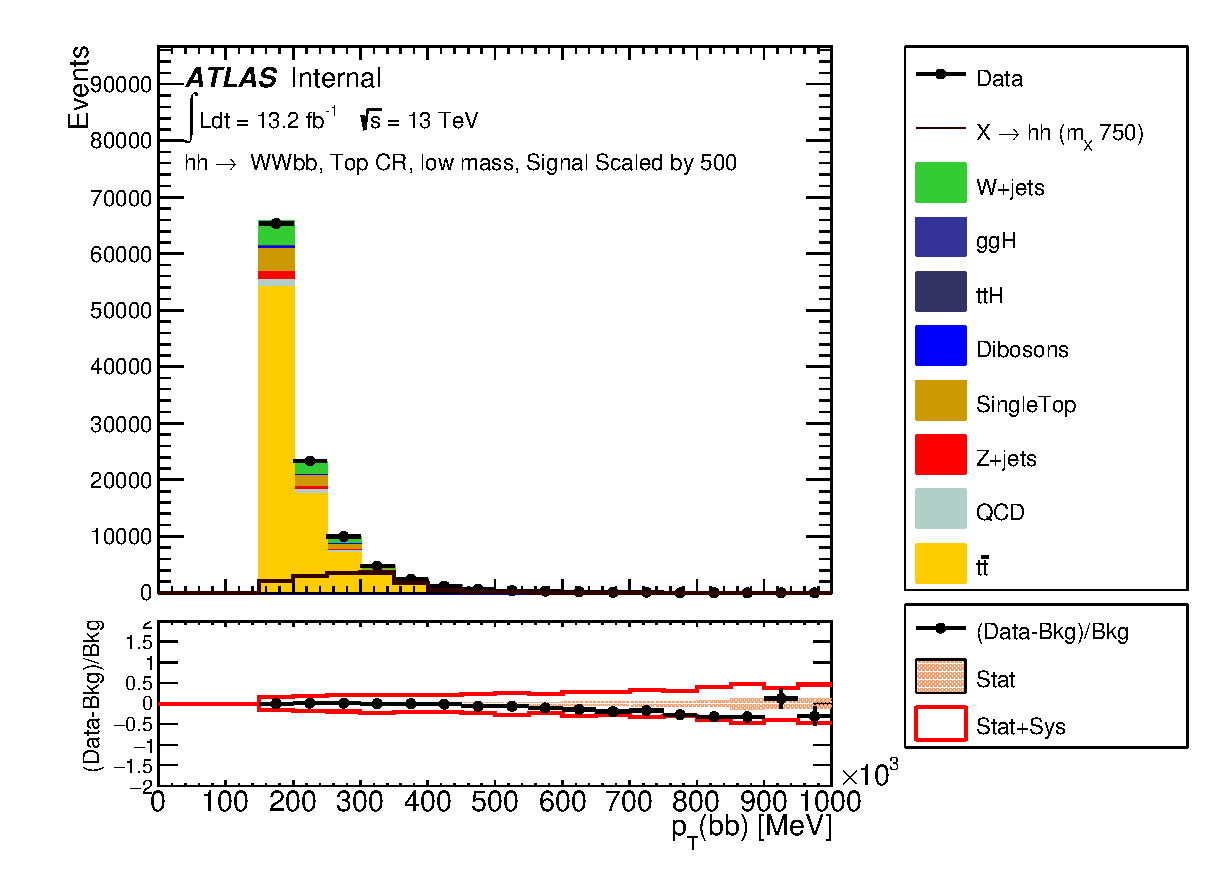
\includegraphics[height=60mm]{chapters/dihiggs/figures/ControlPlots/CR1/C_opt700_bbpt150_bbPt.eps} 
		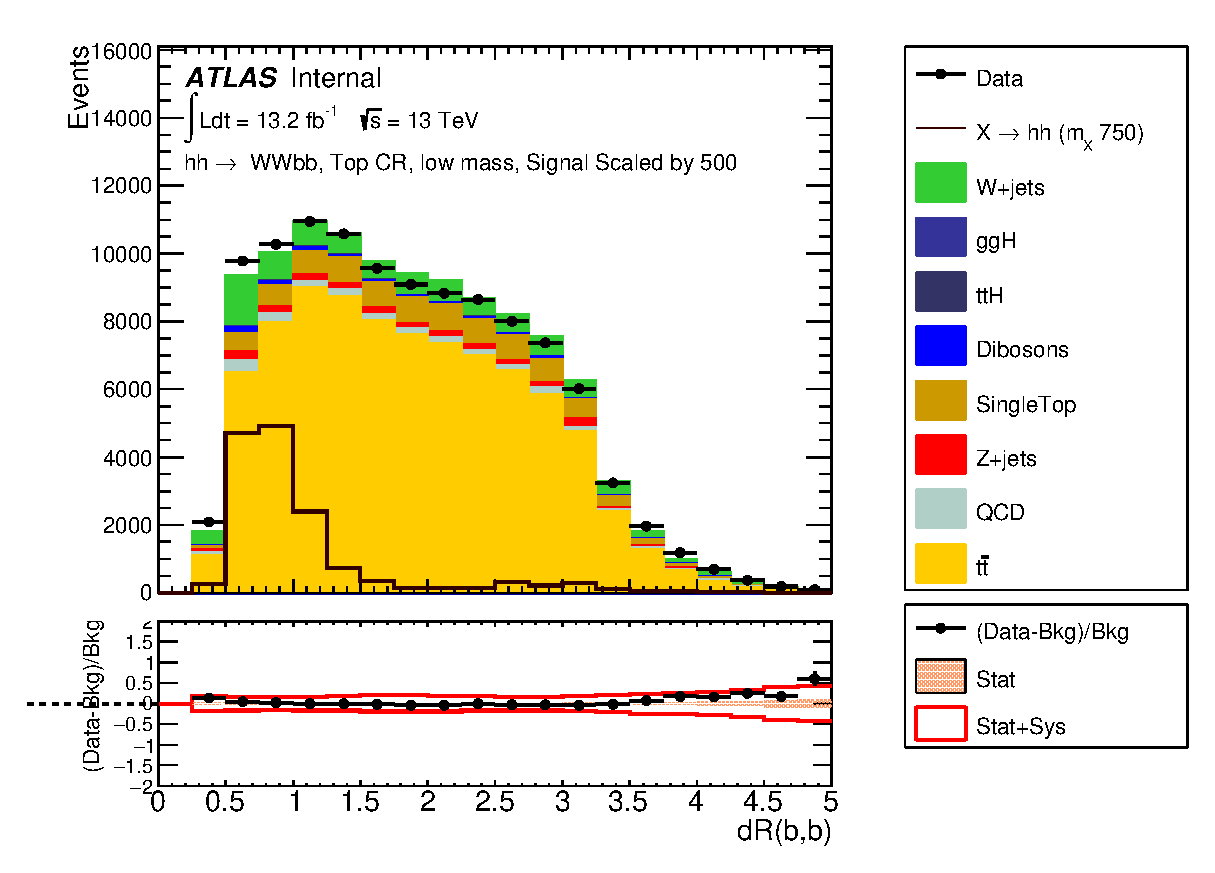
\includegraphics[height=60mm]{chapters/dihiggs/figures/ControlPlots/CR1/C_opt700_bbpt150_drbb.eps} 
		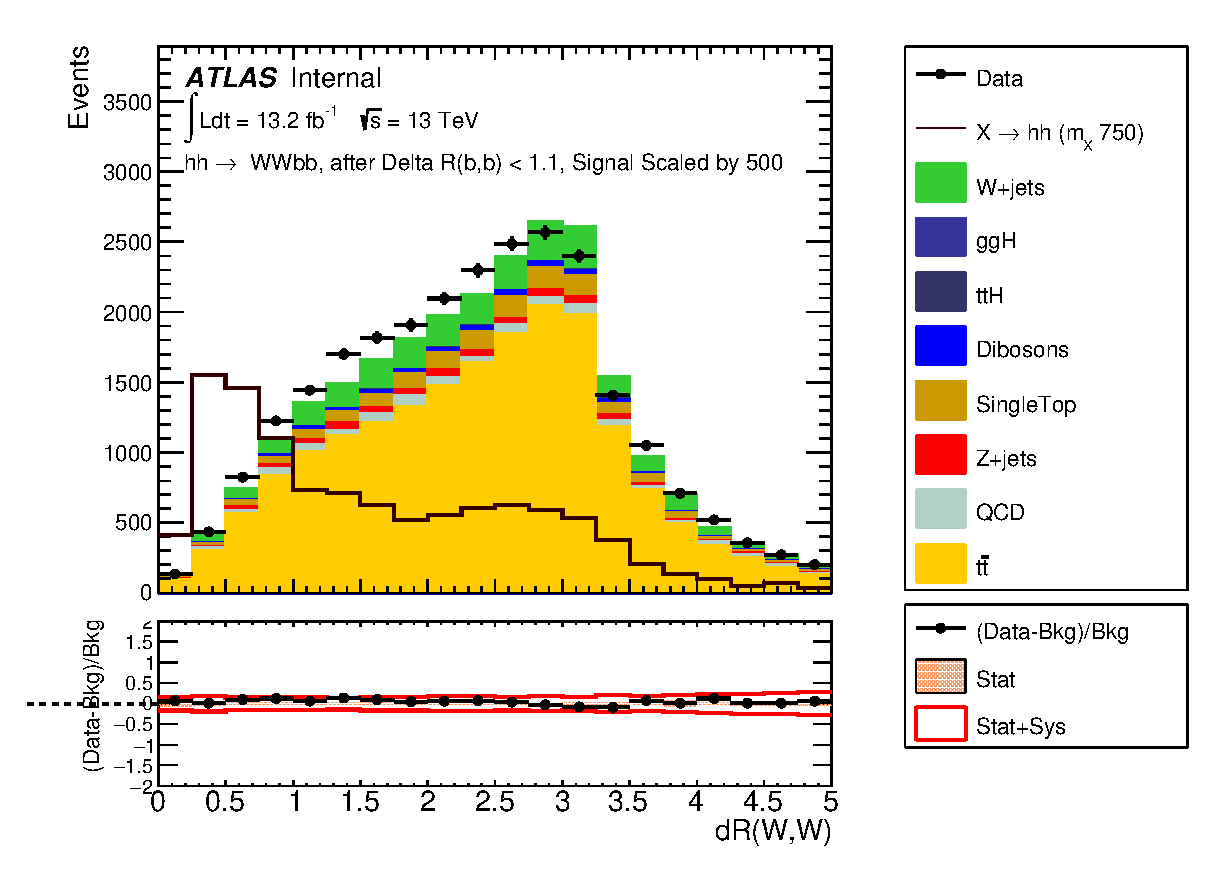
\includegraphics[height=60mm]{chapters/dihiggs/figures/ControlPlots/CR1/C_opt700_bbpt150_drbb11_drww.eps}
		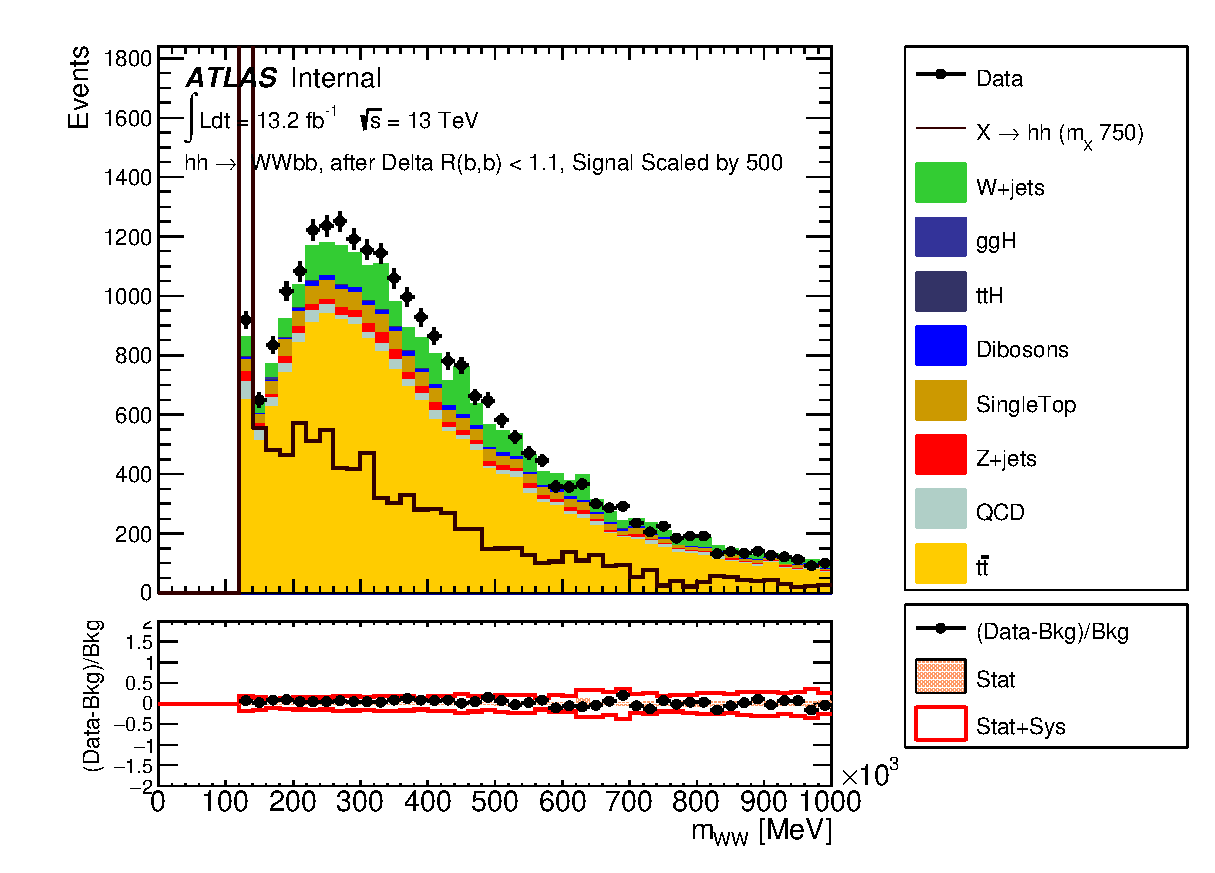
\includegraphics[height=60mm]{chapters/dihiggs/figures/ControlPlots/CR1/C_opt700_bbpt150_drbb11_WWMass.eps} 
		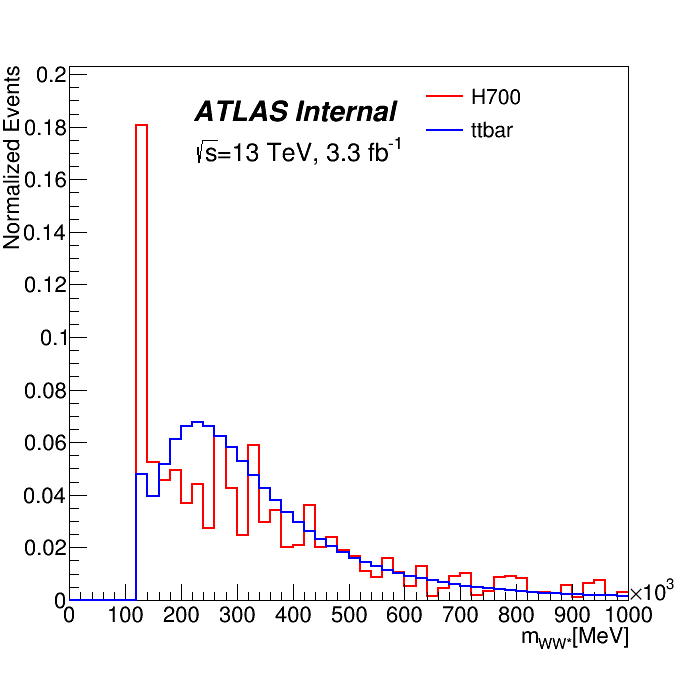
\includegraphics[height=60mm]{chapters/dihiggs/figures/Presel_WWMass.png} 
		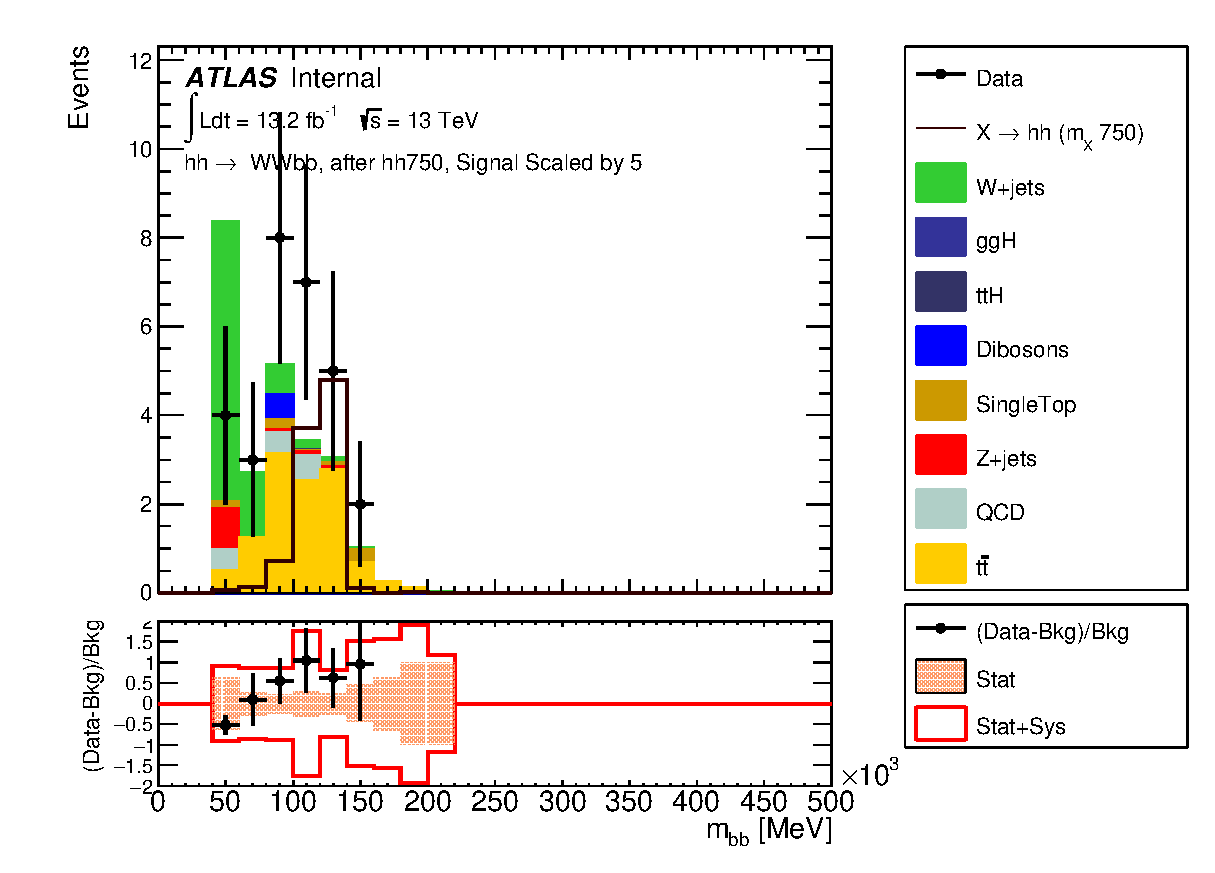
\includegraphics[height=60mm]{chapters/dihiggs/figures/ControlPlots/CR1/C_opt700_bbpt150_drbb11_drww09_mww_hh750_bbMass.eps}
%                 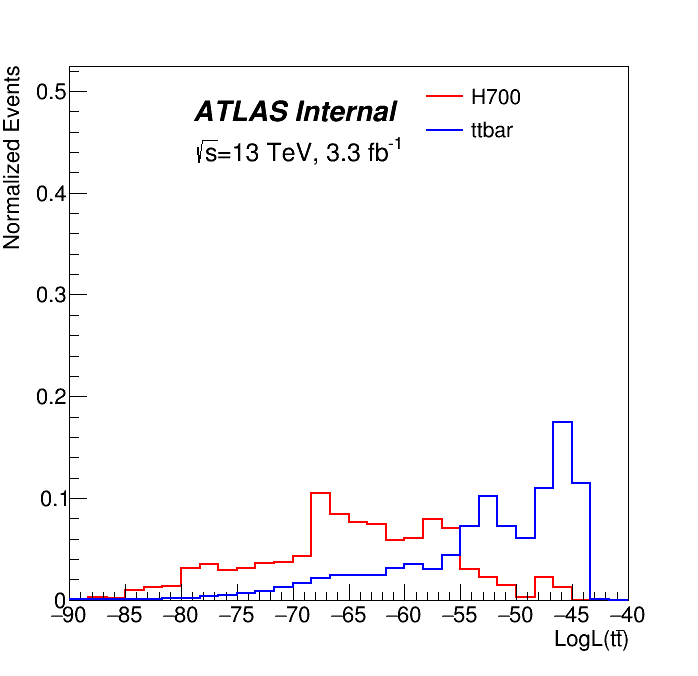
\includegraphics[height=65mm]{chapters/dihiggs/figures/Presel_LogLikelihood_ttbar.png}
	\caption{Event  kinematic distributions at pre-selection stage. The
                 distributions show the main difference between the signal and
                 the background processes.}
	\label{fig:kin_presel}
	\end{center}    
\end{figure}
\fi

\begin{figure}[!h]
\begin{center}
\includegraphics*[width=0.47\textwidth] {chapters/dihiggs/figures/ControlPlots/CR1/C_opt700_bbpt150_bbPt.eps}
\includegraphics*[width=0.47\textwidth] {chapters/dihiggs/figures/ControlPlots/CR1/C_opt700_bbpt150_drbb.eps}
\caption [$\pt(bb)$ in low mass Top CR and $\Delta R(b,b)$ in just before applying cut on it.] {$\pt(bb)$ in low mass Top CR and $\Delta R(b,b)$ in just before applying cut on it. }
\end{center}
\label{fig:topcr_bbpt_drbb}
\end{figure}

\begin{figure}[!h]
\begin{center}
\includegraphics*[width=0.47\textwidth] {chapters/dihiggs/figures/ControlPlots/CR1/C_opt700_bbpt150_drbb11_drww.eps}
\includegraphics*[width=0.47\textwidth] {chapters/dihiggs/figures/ControlPlots/CR1/C_opt700_bbpt150_drbb11_drww09_WWMass.eps}
\caption [$mT$ and $m_{(W,W^{\ast})}$ in low mass selection just before applying cuts on them.] {$mT$ and $m_{(W,W^{\ast})}$ in low mass selection just before applying cuts on them.  }
\end{center}
\label{fig:drww_mww}
\end{figure}

\begin{figure}[!h]
\begin{center}
\includegraphics*[width=0.47\textwidth] {chapters/dihiggs/figures/ControlPlots/CR1/C_opt700_bbpt150_drbb11_drww09_mww_hhMass.eps}
\includegraphics*[width=0.47\textwidth] {chapters/dihiggs/figures/ControlPlots/CR1/C_opt700_bbpt150_drbb11_drww09_mww_hh750_bbMass.eps}
\caption[$m_{hh}$ and $m_{bb}$ in low mass selection just before applying cuts on them.]{$m_{hh}$ and $m_{bb}$ in low mass selection just before applying cuts on them. }
\end{center}
\label{fig:mhh_mbb}
\end{figure}

\begin{figure}[!h]
\begin{center}
\includegraphics*[width=0.47\textwidth] {chapters/dihiggs/figures/ControlPlots/CR2/C_opt2000_bbpt350_bbPt.eps}
\includegraphics*[width=0.47\textwidth] {chapters/dihiggs/figures/ControlPlots/CR2/C_opt2000_bbpt350_WWPt.eps}
\caption [$\pt(bb)$ in high mass top CR and $\pt(WW^{\ast})$ in high mass selection just before applying cut on it.] {$\pt(bb)$ in high mass top CR and $\pt(WW^{\ast})$ in high mass selection just before applying cut on it.  }
\end{center}
\end{figure}


\begin{figure}[!h]
\begin{center}
\includegraphics*[width=0.47\textwidth] {chapters/dihiggs/figures/ControlPlots/CR2/C_opt2000_bbpt350_drww.eps}
\includegraphics*[width=0.47\textwidth] {chapters/dihiggs/figures/ControlPlots/CR2/C_opt2000_bbpt350_wwpt360_drww20_hhMass.eps}
%\caption [$\Delta R(W,W^{\ast})$  and $m_{hh}$ in high mass selection just before applying cut on it.] { $\Delta R(W,W^{\ast})$ and $m_{hh}$ in high mass selection just before applying cut on it. }
\caption[$\Delta R(W,W)$ and $m_{hh}$ in high mass selection just before applying cuts on them.] {$\Delta R(W,W)$ and $m_{hh}$ in high mass selection just before applying cuts on them.}
\end{center}
\end{figure}

\begin{figure}[!h]
\begin{center}
\includegraphics*[width=0.47\textwidth] {chapters/dihiggs/figures/ControlPlots/CR2/C_opt2000_bbpt350_wwpt360_drww20_hh2000above_bbMass.eps}
\caption[$m_{bb}$ in high mass selection just before applying cut on it.]{$m_{bb}$ in high mass selection just before applying cut on it.  }
\end{center}
\label{fig:mbb_high_mass}
\end{figure}

These distributions are shown in Figure~\ref{fig:topcr_bbpt_drbb} through~\ref{fig:mbb_high_mass} at the selection just before the cut on the variable is applied. They are obtained comparing a 750 GeV
signal sample with the full backgrounds. In these figures, signal has been multiplied by a varying scale factor for presentation purpose.  

\subsection{Signal region definitions}
\label{subsec:SR}
The cuts of the selection have been optimised by maximising the Poisson
significance at the end of the selection \footnote{a two step procedure has
been implemented. In the first step each cut is optimised, in the second step,
all cuts are set to their optimal value and cuts are varied one by one to
look for a different optimisation point. Correlation among variables 
could in fact spoil the results obtained at the first step.}. The Poisson
significance formula depends on the absolute yield of expected signal and
background events. For the optimisation formula the ttbar background was
normalised to data with $m_{bb} < 100$ GeV or $m_{bb} > 140$ GeV, 
such region rejects, in fact, the majority of the signal. Two signal
hypotheses have been used in the optimisation: resonant
heavy Higgs with $m_H = 750$ GeV and resonant heavy Higgs with $m_H = 2000$ GeV.
The $750$ GeV and $2000$ GeV signal samples have been normalised to the Run-1 upper limit scaled by the $13/8$ TeV cross section ratio expected from the
PDF luminosity scale of a narrow resonance of that mass. 

The signal regions for the two  reference signal hypotheses are summarised in 
Table~\ref{tab:sig_reg_summary}.

% BBT, Aug 10 2016, removing non-res selection
%\begin{table}
%\begin{center}
%\begin{tabular}{c|c|c|c}
%\hline
% variable  & \multicolumn{3}{c}{cut} \\
% & non res. & $m_H = 700$ GeV &  $m_H = 2000$  GeV\\
%\hline
% $p_T^{bb} >$ (GeV) & 230  & 150 & 350 \\
%$\Delta R^{\rm bb}  <$ & 1.2 & 1.1 & no cut \\
%$p_T^{\rm WW} >$ (GeV) & no cut & no cut & 360 \\
%$\Delta R^{\rm WW} <$ & 1.1 & 0.9 & 2.0 \\
%$m_{\rm WW} <$ (GeV) & 130 & 130 &  no cut \\
%$m_{\rm hh}$ (GeV) & no cut. & 640 - 760 & $> 1800$ \\
%$m_{bb}$ (GeV) & 105-135 & 105-135 & 105-135 \\
%\hline
%\end{tabular}
%\end{center}
%\caption{Event selection optimised for the three different signal hypotheses.} 
%\label{tab:sig_reg_summary}
%\end{table}

\begin{table}
\caption{Event selection for the two different signal hypotheses.}
\label{tab:sig_reg_summary}
\begin{center}
\begin{tabular}{c|c|c|c}
\hline
 variable  & \multicolumn{2}{c}{cut} \\
 & $m_H = 750$ GeV &  $m_H = 2000$  GeV\\
\hline
 $p_T^{bb} >$ (GeV) & 150 & 350 \\
$\Delta R^{\rm bb}  <$ & 1.1 & no cut \\
$p_T^{\rm WW} >$ (GeV) & no cut & 360 \\
$\Delta R^{\rm WW} <$ & 0.9 & 2.0 \\
$m_{\rm WW} <$ (GeV) & 130 &  no cut \\
$m_{\rm hh}$ (GeV) & 680 - 820 & $> 1800$ \\
$m_{bb}$ (GeV) & 105-135 & 105-135 \\
\hline
\end{tabular}
\end{center}
\end{table}

%In order to better exploit all the kinematic constraints available in the $t\bar{t}$ 
%configuration a kinematic fit imposing transverse energy momentum conservation,
%the mass of the top-quark intermediate states and the mass of the $W$ bosons is performed. 
%The kinematic fit starts from pre-selected events and the neutrino longitudinal momentum
%described above. Jets are instead taken in all possible combination and the fit is performed 
%with several jet assignment to the $W$ boson  and top quark (see appendix \ref{subsec:KinFit}).
%The maximum of the likelihood, so the configuration resembling most the $t \bar{t}$ kinematic,  
%is retained, and such value is used to reject the $t \bar{t}$ backgorund with a cut that 
%has been optimised differently for the three signal hypotheses. The full selection has been 
%reoptimised including the kinematic fit cut. The distribution of $Log(L)$ is shown in 
%Figure \ref{fig:logL}.

%\begin{figure}[!hb]

%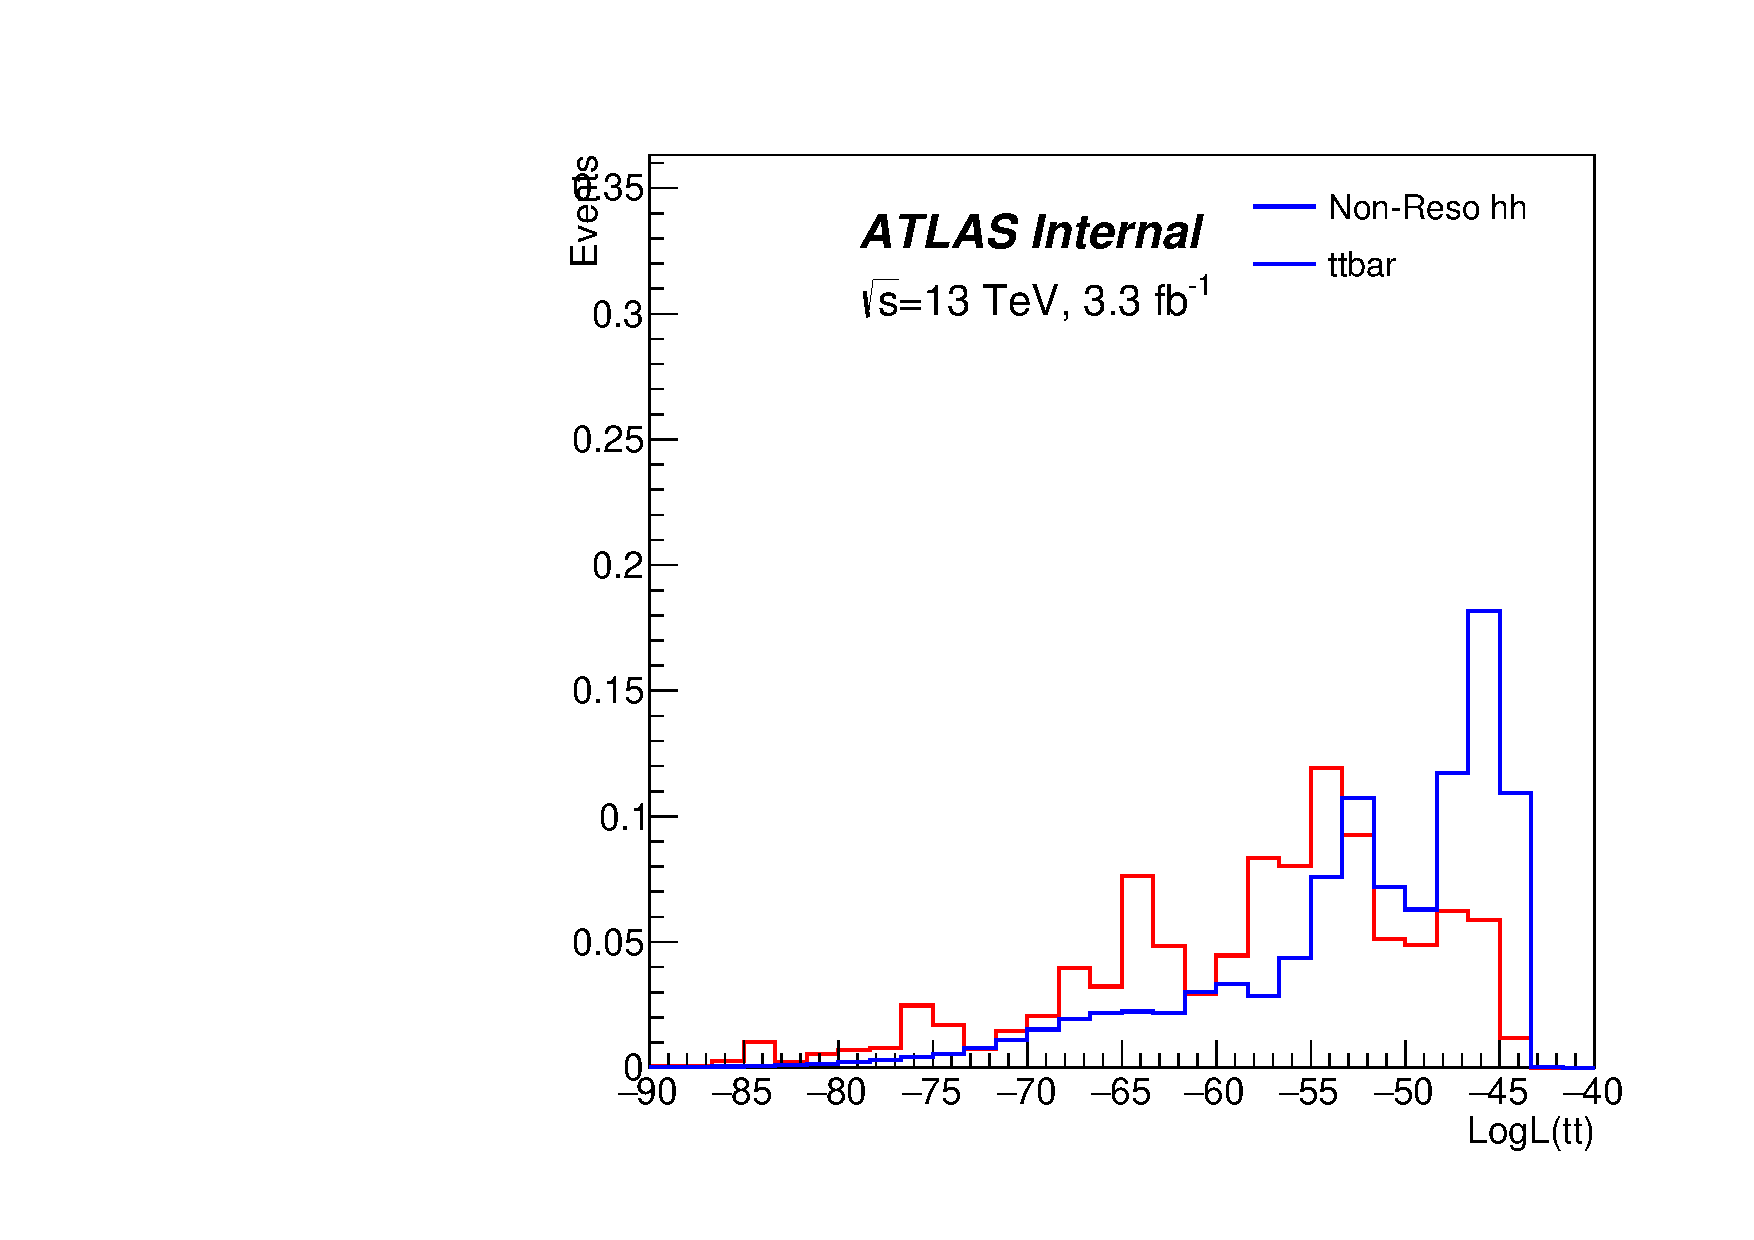
\includegraphics[height=50mm]{chapters/dihiggs/figures/logL_ttbar_hhSM.pdf}
%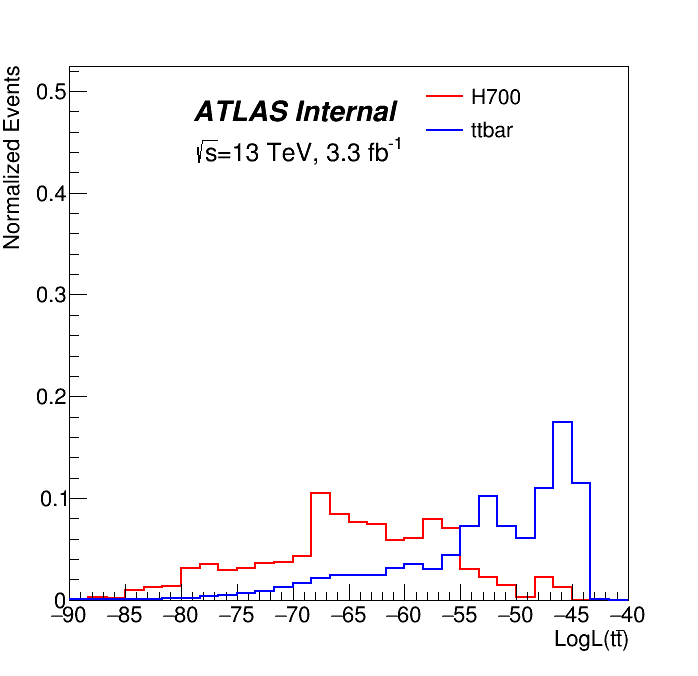
\includegraphics[height=50mm]{chapters/dihiggs/figures/Presel_LogLikelihood_ttbar.png}
%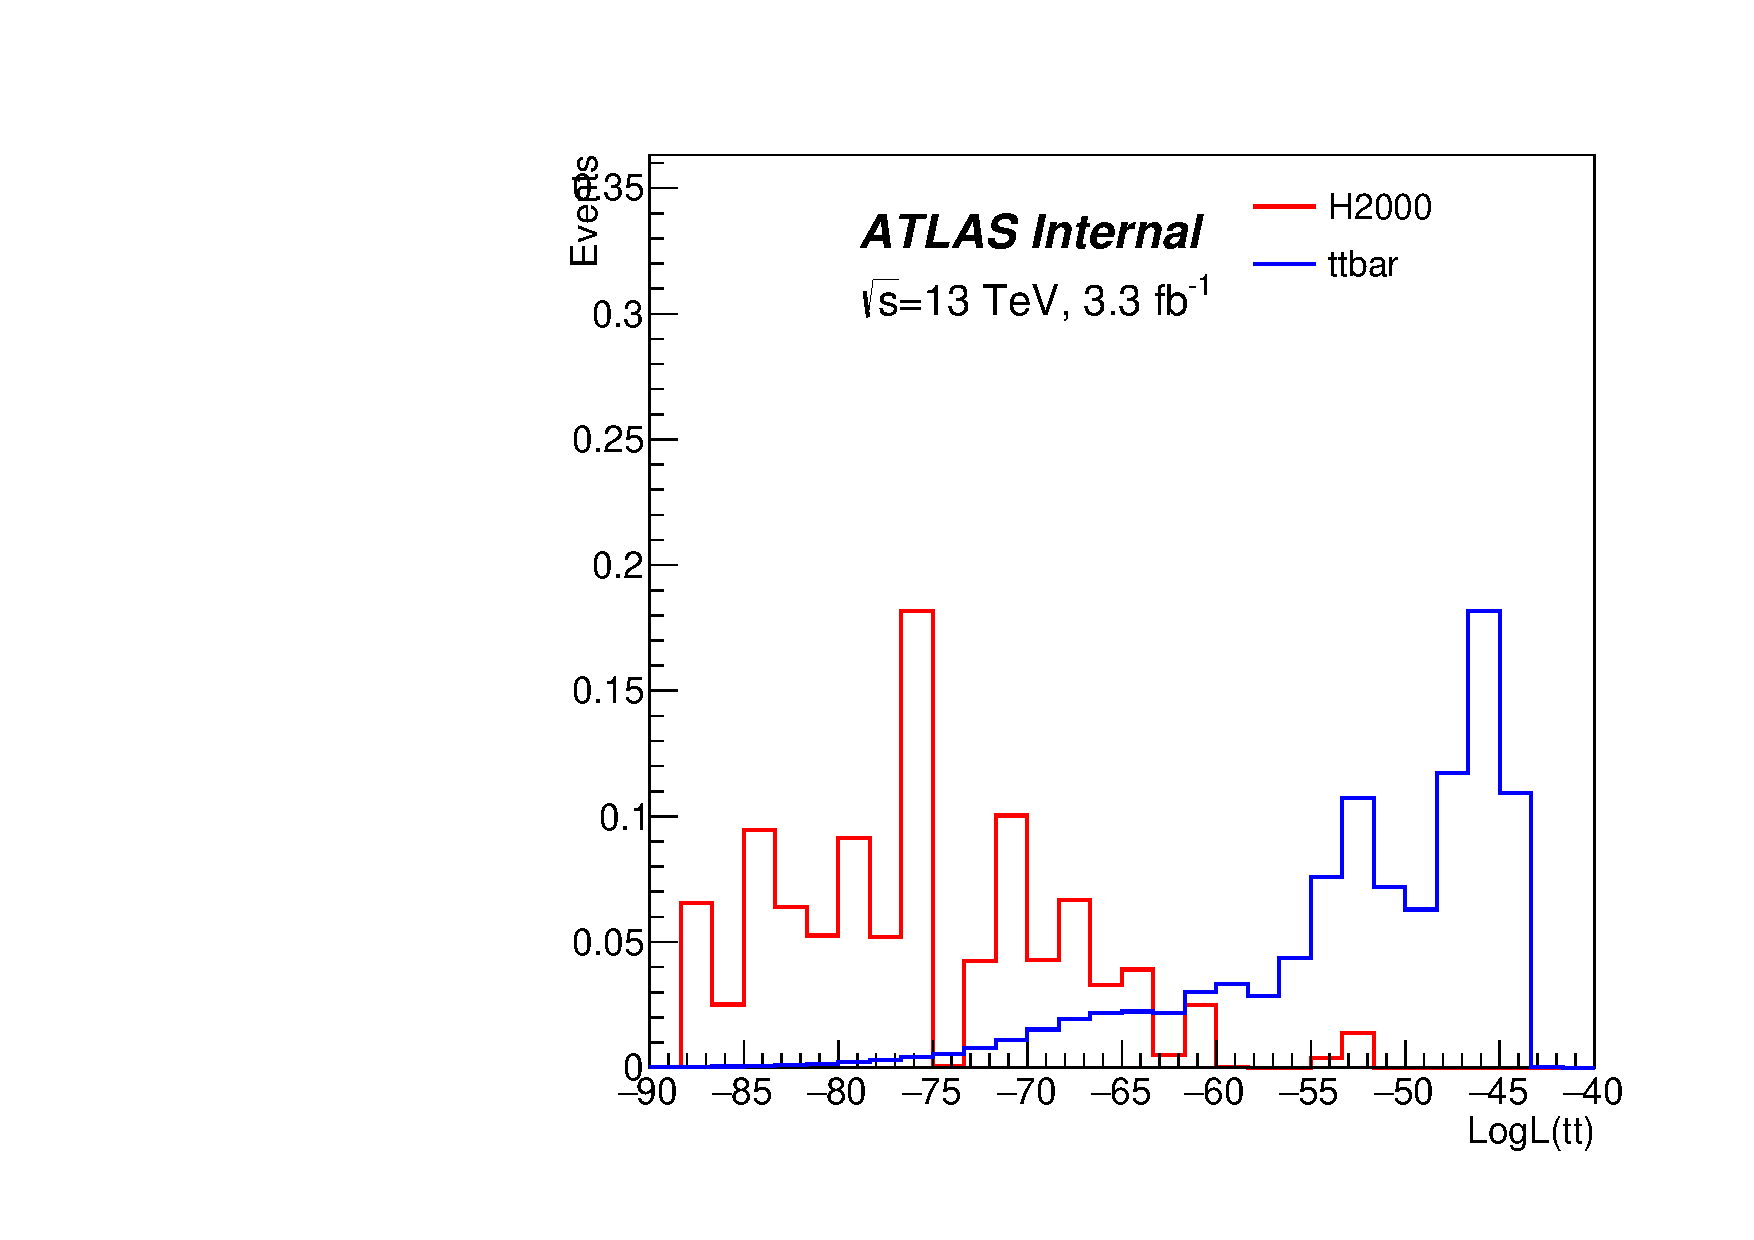
\includegraphics[height=50mm]{chapters/dihiggs/figures/logL_ttbar_Xhh2000.pdf}
%\caption{Log${\rm (Likelihood)}$ distribution of the kinematic fit in
 % the $t\bar{t}$ hypothesis. The distribution is shown for non
%  resonant SM background, for a signal at 700 GeV and 2000 GeV. } \label{fig:logL}
%\end{figure}
%Table \ref{tab:kin_fit_opt} shows the optimised cuts for all signal regions including the kin%ematic 
%fit $t \bar{t}$ rejection.

%\begin{table}
%\begin{center}
%\begin{tabular}{c|c|c|c}
%\hline
% variable  & \multicolumn{3}{c}{cut} \\
% & non res. & $m_H = 700$ GeV &  $m_H = 2000$  \\
%\hline
% $p_T^{bb} >$ (GeV) & 240  & 150 & 350 \\
%$\Delta R^{\rm bb}  <$ & 0.9 & 0.9 & no cut \\
%$p_T^{\rm WW} >$ (GeV) & no cut & no cut & 360 \\
%$\Delta R^{\rm WW} <$ & 1.1 & 0.9 & 2.0 \\
%$m_{\rm WW} <$ (GeV) & 130 & 130 &  no cut \\
%$m_{\rm hh}$ (GeV) & no cut. & 640 - 760 & $> 1800$ \\
%$m_{bb}$ (GeV) & 105-135 & 105-135 & 105-135 \\
%$Log(\rm Likelihood) < $&  - 60 & -60 & -80 \\
%\hline
%\end{tabular}
%\end{center}
%\caption{Event selection optimised for the three different signal hypotheses using the $t\bar{t}$ rejection through kinematic fit.} \label{tab:kin_fit_opt}
%\end{table}


\clearpage
